\documentclass[10pt]{article}
\usepackage{../../local}
\urlstyle{same}

\newcommand{\classcode}{Physics 110B}
\newcommand{\classname}{Electromagnetism and Optics II}
\renewcommand{\maketitle}{%
\hrule height4pt
\large{Eric Du \hfill \classcode}
\newline
\large{HW 10} \Large{\hfill \classname \hfill} \large{\today}
\hrule height4pt \vskip .7em
\small{Header styling inspired by the Berkeley EECS Department: \url{https://eecs.berkeley.edu/}}
\normalsize
}
\linespread{1.2}
\begin{document}
	\maketitle
	\section*{Collaborators}
	I worked with \textbf{Teja Nivarthi} on this assignment. 


	\section*{Problem 1} 
	Find the angle \( \theta_\text{max} \) at which the maximum radiation is emitted, in Ex. 11.3 (Fig.
	11.13). Show that for ultrarelativistic speeds (\( v \) close to \( c \)), 
	\[
		\theta_\text{max} \approx \sqrt{( 1 - \beta)} / 2
	\]
	What is the intensity of the radiation in this maximal direction (in the ultrarelativistic case) in
	proportion to the same quantity for a particle instantaneously at rest? Give your answer in terms of \(
	\gamma \).  

	\begin{solution}
		For this problem, we use the value of \( \dv{P}{\Omega} \), equation 11.74:
		\[
			\dv{P}{\Omega} = \frac{\mu_0 q^2 a^2}{16 \pi^2 c} \frac{\sin^2 \theta}{(1 - \beta \cos \theta)^{5}}
		\]
		We can differentiate this with respect to \( \theta \) to find \( \theta_\text{max} \):
		\[
			0 = \pdv{\theta} \dv{P}{\Omega} = \frac{\mu_0 q^2 a^2}{16 \pi^2 c} \frac{2 \sin \theta \cos \theta (1
			- \beta \cos \theta)^{5} - \sin^2 \theta \cdot 5(1 - \beta \cos \theta)^{4} (\beta \sin
		\theta)}{(1 - \beta \cos \theta)^{10}}
		\]
		Simplifying this down, we find the following equation:
		\[
			3 \cos^2 \theta + 2 \cos \theta - 5 \beta = 0
		\]
		This is quadratic in \( \cos \theta \), so we can use the quadratic formula:
		\[
			\cos \theta = \frac{-1 \pm \sqrt{1 + 15 \beta^2}}{3 \beta}
		\]
		Now, we require that in the case where \( \beta \to 0 \), that the maximum is \( \theta =
		\frac{\pi}{2} \), since we know that in this limit the radiation is maximally radiated in the
		direction perpendicular to the motion of the particle. As such, we pick the solution which is
		consistent to this end, and so we choose the positive sign here. Thus, \( \theta_\text{max} \) is:
		\[
			\theta_\text{max} = \cos ^{-1}\left( \frac{\sqrt{1 + 15 \beta^2} - 1}{3 \beta} \right)
		\]
		We can simplify this by Taylor expanding the argument around \( \beta \approx 1 \), which gives:
		\[
			\theta_\text{max} = \cos ^{-1}\left( 1 + \frac{\beta - 1}{4} \right) \implies \cos \theta_\text{max}
			= 1 + \frac{\beta - 1}{4}
		\]
		Since the quantity on the right is very close to 1, we can infer that \( \theta_\text{max} \approx 0
		\), so we can Taylor expand the cosine:
		\[
			1 - \frac{\theta^2}{2} = 1 + \frac{\beta - 1}{4} \implies \theta^2 =\frac{1 - \beta}{2}
		\]
		This gives us the solution:
		\[
			\theta_\text{max} \approx \sqrt{\frac{1 - \beta}{2}}
		\]
		We can't really take the 2 outside of the square root, though it won't really do much for us to take
		it out anyways since the numerator \( \sqrt{1 - \beta} \) is very small anyways, so that gets us the
		final result:
		\[
			\theta_\text{ max} \approx \frac{\sqrt{1 - \beta}}{2}
		\]
	\end{solution}

	\pagebreak
	\section*{Problem 2}
	In Ex. 11.3 we assumed the velocity and acceleration were (instantaneously, at least) \textit{collinear}.
	Carry out the same analysis for the case where they are \textit{perpendicular}. Choose your axes so that
	\( \mathbf{v} \) lies along the \( z \)-axis and \( \mathbf{a} \) along the \( x \)-axis (Fig. 11.14), so
	that \( \mathbf{v} = v \mathbf{\hat{z}} \), \( \mathbf{a} = a \mathbf{\hat{x}} \) and \( \hat{\brcurs} =
	\sin \theta \cos \phi \mathbf{\hat{x}}+ \sin \theta \sin \phi \mathbf{\hat{y}} + \cos \theta
	\mathbf{\hat{z}}\). Check that \( P \) is consistent with the Lienard formula. [\textit{Answer:}
	\[
		\dv{P}{\Omega} = \frac{\mu_0q^2 a^2}{15\pi^2 c} \frac{\left[ (1 - \beta \cos \theta)^2 - (1 -
		\beta^2) \sin^2 \theta \cos^2 \phi \right]}{(1 - \beta \cos \theta)^{5}}, \quad P = \frac{\mu_0 q^2
		a^2 \gamma^{4}}{6 \pi c}
	\]
	For relativistic velocities (\( \beta \approx 1 \)) the radiation is again sharply peaked in the forward
	direction (Fig. 11.15). The most important application of these is to \textit{circular} motion -- in this
	case the radiation is called \textbf{synchrotron radiation.} For a relativistic electron, the radiation
	sweeps around like a locomotive's headlight as the particle moves.]

	\begin{solution}
		We will follow a similar analysis to what we did in 11.3. First, we write out \( \dv{P}{\Omega} \):
		\[
			\dv{P}{\Omega} = \frac{q^2c^2}{16 \pi^2 \epsilon_0} \frac{|\hat{\brcurs} \times (\mathbf{u}
			\times \mathbf{a})|^2}{(\hat{\brcurs} \cdot \mathbf{u})^{5}}
		\]
		Here, we have \( \mathbf{u} = c \hat{\brcurs} - \mathbf{v} \), and since we choose \( \mathbf{v} \)
		in the \( z \)-axis, then we write \( \mathbf{u} = c \hat{\brcurs} - v \mathbf{\hat{z}} \). Now,
		using the vector triple product, we have:
		\[
			\hat{\brcurs} \times (\mathbf{u} \times \mathbf{a}) = (\hat{\brcurs} \cdot \mathbf{a}) \mathbf{u}
			- (\hat{\brcurs} \cdot \mathbf{u}) \mathbf{a}
		\]
		We need this quantity squared:
		\[
			|\hat{\brcurs} \times (\mathbf{u} \times \mathbf{a})|^2 = (\hat{\brcurs} \cdot \mathbf{a})^2 u^2
			- 2(\hat{\brcurs} \cdot \mathbf{a}) (\hat{\brcurs} \cdot \mathbf{u}) (\mathbf{u} \cdot
			\mathbf{a}) + (\hat{\brcurs} \cdot \mathbf{u})^2 a^2
		\]
		Now, \( (\hat{\brcurs} \cdot \mathbf{a})^2 = a^2 \sin^2 \theta \cos^2 \phi \), \( \hat{\brcurs} \cdot
		\mathbf{u} = c - v \cos \theta \) and \( \mathbf{u} \cdot \mathbf{a} = ac \sin \theta \cos \phi \)
		just from computing the dot products. So, we can put this all together and plug this in to get, after
		some algebra:
		\[
			\dv{P}{\Omega} = \frac{\mu_0 q^2 a^2}{16 \pi^2 c} \frac{(1 - \beta \cos \theta)^2 - (1 - \beta^2)
			\sin^2 \theta \cos^2 \phi}{(1 - \beta \cos \theta)^{5}}
		\]
		Now, we integrate over all angles:
		\[
			P = \frac{\mu_0 q^2 a^2}{16 \pi^2 c} \int_{0}^{2\pi}\int_{0}^{\pi}  \frac{(1 - \beta \cos \theta)^2 - (1 - \beta^2)
			\sin^2 \theta \cos^2 \phi}{(1 - \beta \cos \theta)^{5}} \sin \theta \diff \theta \diff \phi
		\]
		This is also consistent with the "partial answer" given in the problem statement. This is a big
		integral, so we resort to Mathematica (regrettably so, but my patience with integrals is
		\textit{extremely} limited):
		\[
			P = \frac{\mu_0 q^2 a^2}{16 \pi^2 c} \frac{8\pi}{3(-1 + \beta^2)^2} 
			= \frac{\mu_0 q^2 a^2}{16 \pi^2 c}  \frac{8\pi}{3(1 - \beta^2)^2}
		\]
		Now, using \( \gamma = 1 / \sqrt{1 - \beta^2} \), then we can write:
		\[
			P = \frac{\mu_0 q^2 a^2\gamma^{4}}{6 \pi c}
		\]
		this is also consistent with the partial answer for \( P \) we got from the problem statement.
		Lienard's formula is:
		\[
			P = \frac{\mu_0 q^2 \gamma^{6}}{6 \pi c}\left( a^2 - \left|\frac{\mathbf{v} \times
			\mathbf{a}}{c}\right|^2 \right)
		\]
		Here, \( \mathbf{v} \times \mathbf{a} = va \mathbf{\hat{y}} \), so:
		\[
			a^2  - \left| \frac{\mathbf{v} \times \mathbf{a}}{c} \right|^2 = a^2 - \frac{v^2 a^2}{c^2} =
			a^2\left( 1 - \frac{v^2}{c^2} \right) = \frac{a^2}{\gamma^2}
		\]
		And now putting this all back into \( P \):
		\[
			P = \frac{\mu_0 q^2 \gamma^{6}}{6 \pi c} \frac{a^2}{\gamma^2} = \frac{\mu_0 q^2 a^2 \gamma^{4}}{6
			\pi c}
		\]
		so indeed they are consistent.
	\end{solution}
	
	\pagebreak
	\section*{Problem 3}
	With the inclusion of the radiation reaction force (Eq. 11.80), Newton's second law for a charged particle
	becomes 
	\[
		a = \tau \dot a + \frac{F}{m}
	\]
	where \( F \) is the external force acting on a particle. 
	\begin{enumerate}[label=(\alph*)]
		\item In contrast to an \textit{uncharged} particle (\( a = F / m \)), acceleration (like position
			and velocity) must now be a \textit{continuous} function of time, even if the force changes
			abruptly. (Physically, the radiation reaction damps out any rapid change in \( a \).)
			\textit{Prove} that \( a \) is continuous at any time \( t \), by integrating the equation of
			motion from \( (t - \epsilon) \) to \( (t + \epsilon) \) and taking the limit \( \epsilon \to 0 \). 

			\begin{solution}
				Integrating the equation of motion from an interval \( t - \epsilon \) to \( t + \epsilon \),
				we get:
				\[
					\int_{t - \epsilon}^{t + \epsilon} a \diff t = \tau \int_{t - \epsilon}^{t + \epsilon}
					\dv{a}{t} \diff t + \int_{t - \epsilon}^{t + \epsilon} \frac{F}{m} \diff t
				\]
				So, we get:
				\[
					v(t + \epsilon) - v(t - \epsilon) = \tau (a(t + \epsilon) - a(t - \epsilon)) + \frac{2
					\epsilon \mean{F}}{m}
				\]
				We use \( \mean{F} \) in this case because in general \( F \) can vary over time. Now, when
				\( \epsilon \to 0 \), then the left hand side goes to zero and so does the force term, so
				we're left with:
				\[
					\tau (a(t + \epsilon) - a(t - \epsilon)) = 0 
				\]
				and from here we're forced to conclude that \( a(t + \epsilon) = a(t - \epsilon) \), meaning
				that \( a \) must be continuous. 
			\end{solution}
		\item A particle is subjected to a constant force \( F \), beginning at time \( t = 0 \) and lasting
			until time \( T \). Find the most general solution \( a(t) \) to the equation of motion in each
			of the following three periods: (i) \( t < 0 \), (ii) \( 0 < t < T \), (iii) \( t > T \). 

			\begin{solution}
				At \( t < 0 \), there is no force, so the differential equation is just \( a = \tau \dot a
				\), so we can guess an ansats of \( e^{\lambda t} \) and infer that \( \lambda = 1 / \tau \),
				so the solution is:
				\[
					a(t) = A e^{t / \tau}
				\]
				From \( 0 < t < T \), we now have a nonzero \( F \), so the differential equation becomes:
				\[
					a = \tau \dot a + \frac{F}{m}
				\]
				This is the same differential equation as the previous one, except we now just add a constant
				term, so we have:
				\[
					a(t) = B e^{t / \tau} + \frac{F}{m}
				\]
				In the region \( t > T \), the differential equation reverts back to the same one as regime
				(i), so:
				\[
					a(t) = C e^{t / \tau}
				\]
			\end{solution}
		\item Impose the continuity condition (a) at \( t = 0 \) and \( t = T \). Show that you can
			\textit{either} eliminate the runaway in region (iii) \textit{or} avoid preacceleration region in
			region (i), but not both. 

			\begin{solution}
				Imposing the continuity at \( t = 0 \), then we get:
				\[
					A = B + \frac{F}{m}
				\]
				and at \( t = T \), we get:
				\[
					B e^{T / \tau} + \frac{F}{m} = C e^{T / \tau}
				\]
				To eliminate the runaway in region (iii), then we require \( C = 0 \), So therefore, this
				forces:
				\[
					B = -\frac{F}{m}e^{ - T / \tau}
				\]
				To eliminate preacceleration we set \( A = 0 \), and thus:
				\[
					B = -\frac{F}{m}
				\]
				These two equations are not equal, and thus we cannot eliminate both at the same time. 
			\end{solution}
		\item If you choose to eliminate the runaway, what is the acceleration as a function of time, in each
			interval? How about the velocity? (The latter must, of course, be continuous at \( t = 0 \) and \(
			t = T\).) Assume the particle was originally at rest: \( v(-\infty) = 0 \).

			\begin{solution}
				If we choose to eliminate the runaway, then we choose \( C = 0 \), and consequently we choose
				\( B = -\frac{F}{m}e^{-T / \tau} \). So:
				\[
					A = B + \frac{F}{m} = -\frac{F}{m}e^{-T / \tau} + \frac{F}{m} = \frac{F}{m}\left( 1 -
					e^{-T / \tau} \right)
				\]
				and thus in \( t < 0 \):
				\[
					a(t) = \frac{F}{m}\left( 1 - e^{-T / \tau} \right) e^{t / \tau}
				\]
				In region (ii), we have:
				\[
					a(t) = -\frac{F}{m}e^{-T / \tau}e^{t / \tau} + \frac{F}{m} = \frac{F}{m}\left( 1 - e^{(t
					- T) / \tau} \right)
				\]
				Of course, \( a(t) = 0 \) in region (iii). The velocity as a function of time is just the
				integral of this. In region (i), the velocity is then:
				\[
					v(t) = \frac{F}{m}\left( 1 - e^{- T / \tau} \right) \int e^{t / \tau}\diff t = \frac{F
					\tau}{m} \left( 1 - e^{-T / \tau} \right)e^{t / \tau} + C_1
				\]
				Assuming that \( v(-\infty) = 0 \), then this implies that \( C_1 = 0 \). For region (ii), the
				integral is:
				\[
					v(t) = \frac{F}{m} \int 1 - e^{(t - T)/\tau} \diff t = \frac{F}{m}\left( t - \tau e^{(t - T) /
					\tau} \right) + C_2
				\]
				To determine \( C_2 \), we use the value at \( t = 0 \):
				\[
					\frac{F \tau}{m}\left( 1 - e^{-T / \tau} \right) = \frac{F}{m}\left( -\tau e^{-T / \tau}
					\right) + C_2 \implies C_2 = \frac{F \tau}{m}
				\]
				For region (iii), the acceleration is zero, so the velocity is constant from here onwards.
				Its velocity is going to be the same velocity as that at the end of region (ii):
				\[
					v(t) = \frac{FT}{m}
				\]
			\end{solution}
		\item Plot \( a(t) \) and \( v(t) \), both for an uncharged particle and for a (nonrunaway) charged
			particle, subject to this force. 

			\begin{solution}
				I plotted this in Mathematica, the velocity and acceleration. I set constants like \( F, m,
				\tau \) to equal 1 so that they may be plotted properly. For the charged particle, we have:
				\begin{center}
					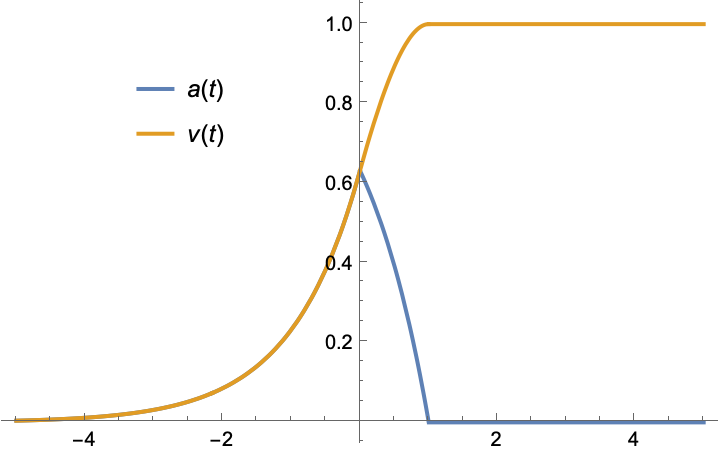
\includegraphics[scale=0.5]{q3e1.png}
				\end{center}
				For the uncharged particle, it just experiences a force \( \frac{F}{m} \) for the duration of
				the interval \( T \), so its graph looks like:
				\begin{center}
					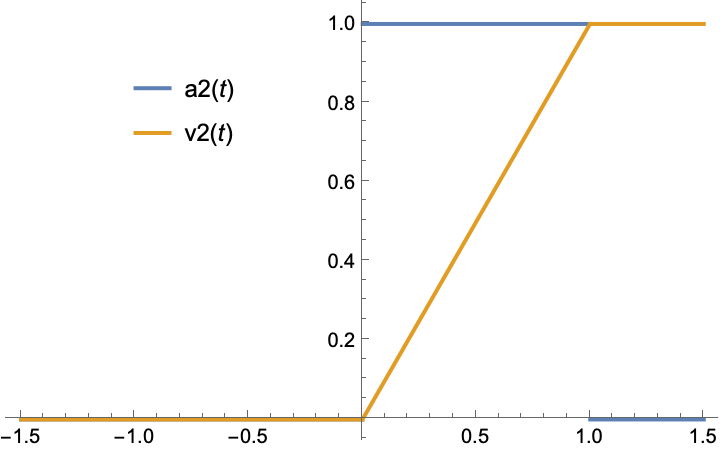
\includegraphics[scale=0.5]{q3e2.png}
				\end{center}
				Here, the differences between a charged and uncharged particle are very clear, as the
				uncharged particle has no preacceleration/runaway but the charged particle could. 
			\end{solution}
	\end{enumerate}
\end{document}
